\title{Assignment 2.2}
\author{
        Pradyot Prakash - 130050008
            \\
        Utkarsh Mall - 130050037
			\\
		Samarth Mishra - 130260018
}
\date{\today}
\documentclass[11pt]{article}
\usepackage[left=2.5cm,top=2cm,right=2.5cm,bottom=2cm,bindingoffset=0.5cm]{geometry}
\usepackage{graphicx}
\usepackage{siunitx}
\usepackage[section]{placeins}
\graphicspath{ {../images/} }
\renewcommand\thesubsection{\Alph{subsection}}
\begin{document}
\maketitle

\subsection{Inverse Radon}
\begin{figure}[h]
\centering
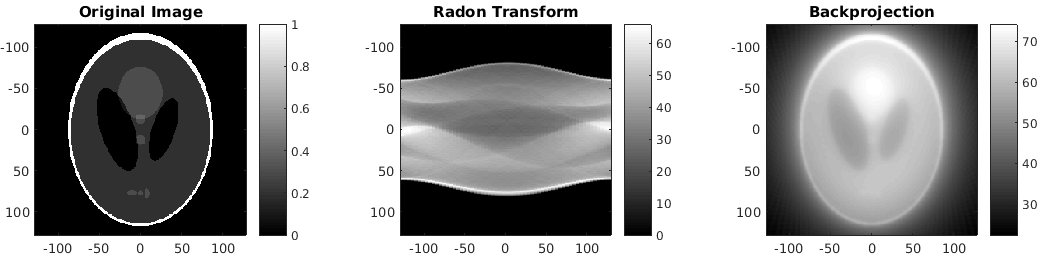
\includegraphics[scale=0.4]{iradonWithoutFilter}
\caption{Shepp Logan Phantom Image, its Radon transform and back-projection of this Radon transform}
\end{figure}

Figure 2 shows the results of applying back projection on filtered radon transforms.
The Images reconstructed by filtered backprojections has artifacts because of discretization.
As the filter changes from Ram-Lak to Shepp-Logan to Cosine the resultant resconstruction become more and more smooth.
As CutOff frequency decreases, more and more high freqency signal removed as a result of artifacts are getting reduced from reconstructed image.

\begin{figure}[h]
\centering
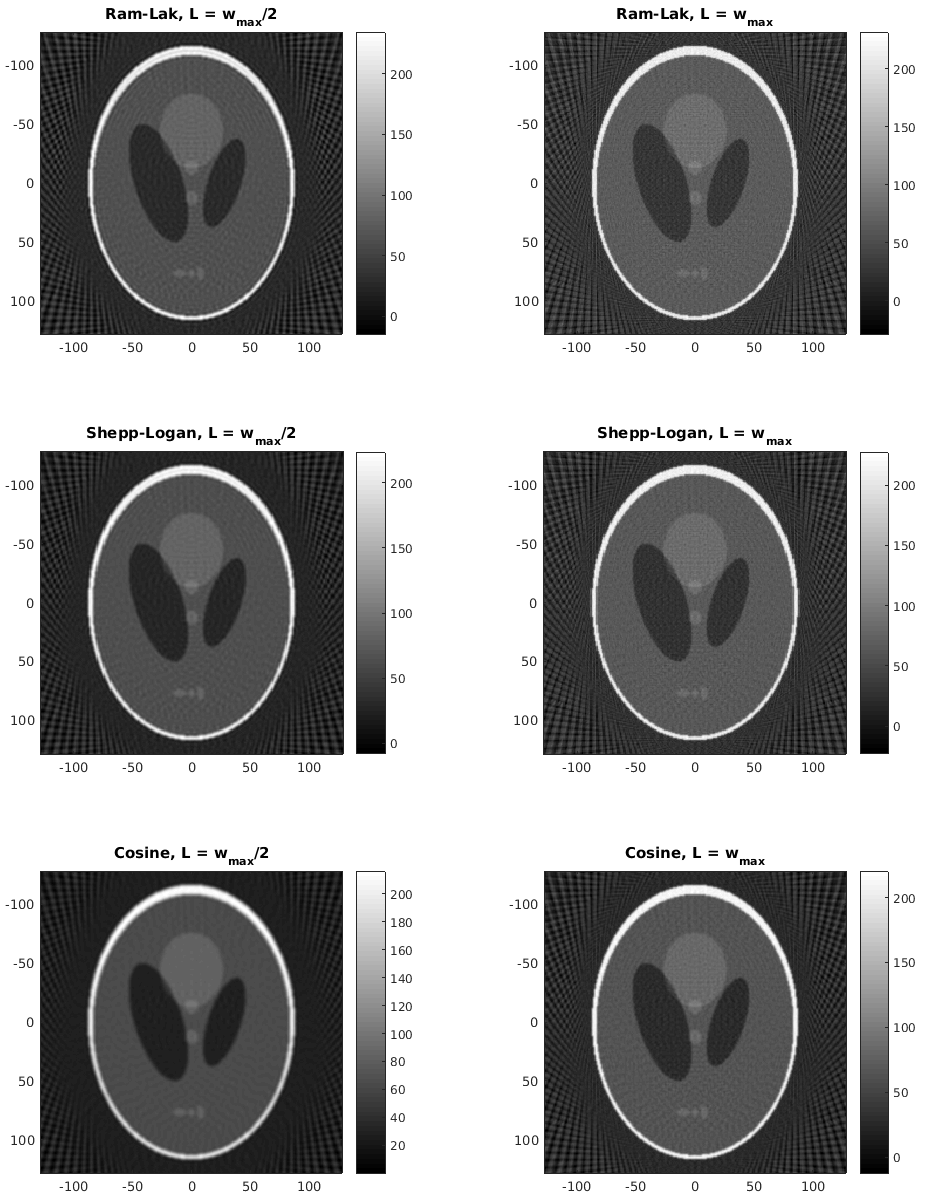
\includegraphics[scale=0.5]{iradon}
\caption{Filtered Back-projection with different filters}
\end{figure}

\subsection{Effect of Blurring}
\begin{table}[!h]
\begin{center}
  \begin{tabular}{ | l | r |}
    \hline
    RRMSE & Value \\
    \hline
    $S_{0}$ & 0.815184 \\
	$S_{1}$ & 0.526613 \\
	$S_{5}$ & 0.066342 \\ \hline
  \end{tabular}
\end{center}
\caption[Table caption text]{RRMSE values for the reconstructed image at various level of blurring}
\end{table}
Higher the smoothing lower is the reconstruction error as shown in Table 1.
Blurring the image smoothes out the discretization noise, as a result of which the reconstruction of more smoothed out image
matches more and more with actual image.

Figure 3 and 4 show the blurred images and their respective recontructions from Radon transform

\begin{figure}[!h]
\centering
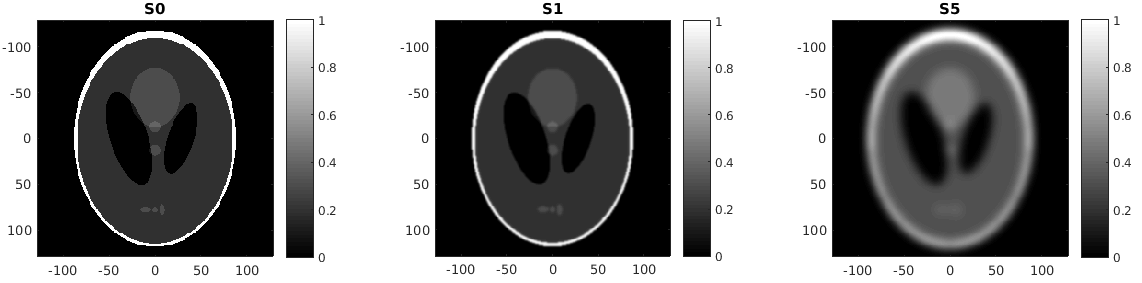
\includegraphics[scale=0.4]{S015}
\caption{Shepp Logan Phantom Image, and its blurred version with standard deviation 1 and 5 pixel width respectively}
\end{figure}

\begin{figure}[!h]
\centering
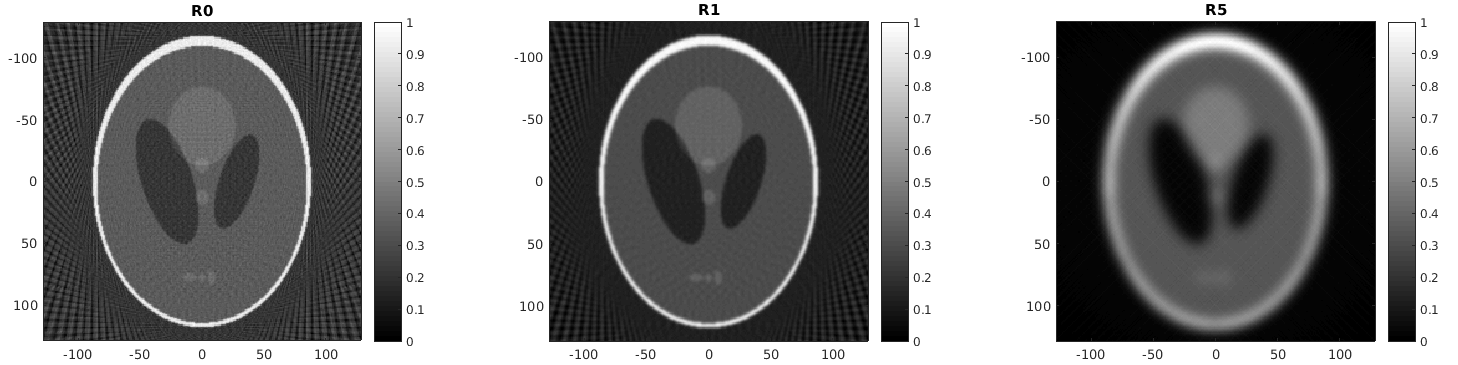
\includegraphics[scale=0.3]{R015}
\caption{Image reconstructed from radon transform of above images}
\end{figure}

\FloatBarrier
\subsection{RRMSE vs L}
When L(Cutoff frequency) is small and close to zero the filter attenuates very low frequencies along with high frequencies as a results of which frequencies consising if useful information goes to zero, hence the error rates are very high.

On the other end when L is large the high frequencies contributing as noise do not get attenuated and increases the reconstruction error.

The RRMSE is minimum somewhere in between $0$ and $w_{max}$. In highly blurred images because the high frequency signals are already attenuated the RRMSE does not increase by large amount after reaching minima as shown in Figure 7.
\begin{figure}[!h]
\centering
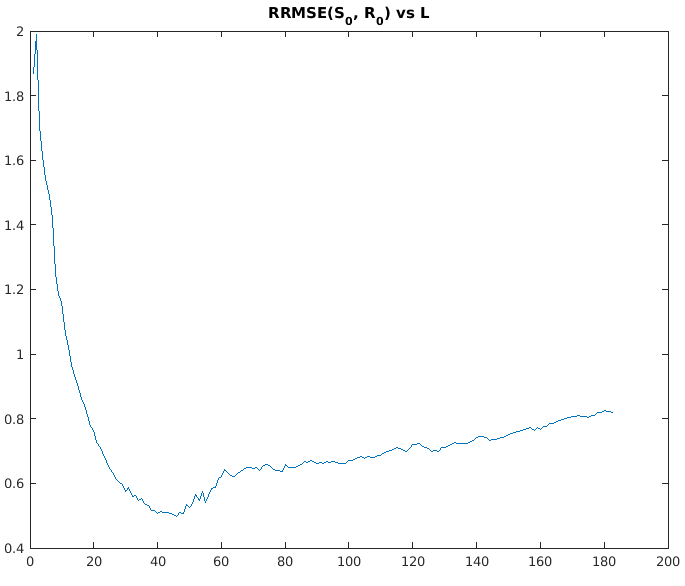
\includegraphics[scale=0.45]{RRMSE0}
\caption{Shepp-Logan Phantom Image's Radon transform with $\Delta s = 0.5,1,3$ respectively}
\end{figure}
\begin{figure}[h]
\centering
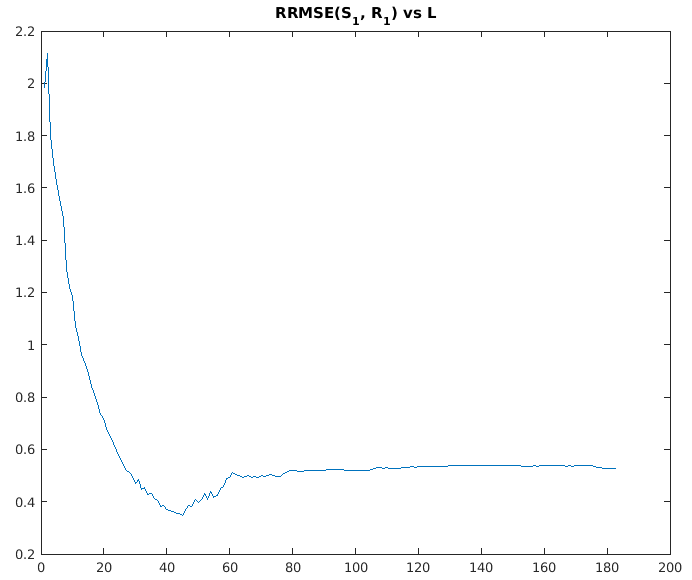
\includegraphics[scale=0.4]{RRMSE1}
\caption{Shepp-Logan Phantom Image's Radon transform Intesity along $\theta=0^{0} $ and $\theta=90^{0} $ with $\Delta s = 0.5,1,3$ respectively}
\end{figure}
\begin{figure}[h]
\centering
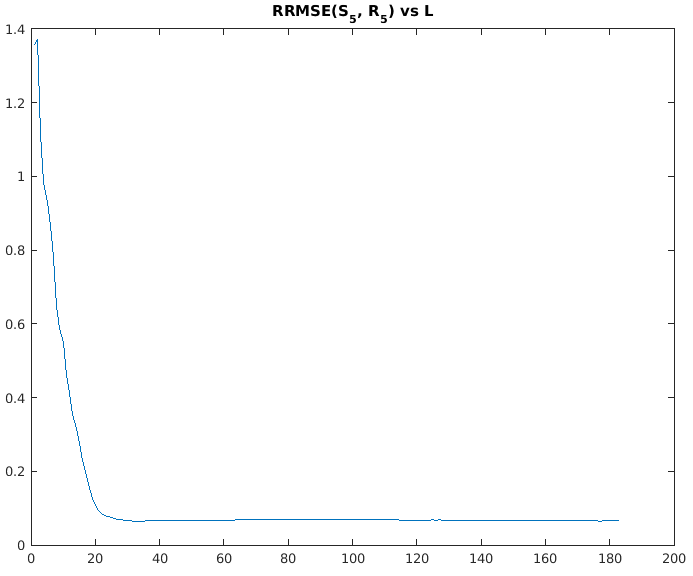
\includegraphics[scale=0.4]{RRMSE5}
\caption{Shepp-Logan Phantom Image's Radon transform Intesity along $\theta=0^{0} $ and $\theta=90^{0} $ with $\Delta s = 0.5,1,3$ respectively}
\end{figure}
\end{document}
